\documentclass[11pt,twoside]{article}

\usepackage[margin=2.5cm]{geometry}     % Marges instellen
\usepackage[dutch]{babel}               % Voor nederlandstalige hyphenatie (woordsplitsing)
\usepackage{graphicx}         			% Om figuren te kunnen verwerken
\usepackage[utf8]{inputenc}             % Om niet ascii karakters rechtstreeks te kunnen typen
\usepackage{parskip}                    % Om paragrafen met een verticale spatie ipv horizontaal te starten
\usepackage{listings}					% Om code weer te geven
\usepackage{courier}
\usepackage[plainpages=false]{hyperref} % Om hyperlinks te hebben in het pdfdocument.


\graphicspath{{fig/}}

\lstset{language=Python,basicstyle=\footnotesize\ttfamily,breaklines=true,showstringspaces=false}

\title{Inleiding tot Python}
\author{Brecht Baeten}

\begin{document}

	\maketitle

	\section{Wat is Python?}
Python is een open source programmeer taal. Voor ingenieurstoepassingen of wetenschappelijke projecten is Python interessant aangezien er een aantal Python Modules bestaan die hier specifiek op gericht zijn. Deze modules maken het beheren van data of uitvoeren van complexe wiskundige algoritmes zeer eenvoudig, vandaar de populariteit. Python werkt volledig object georiënteerd, dit laat toe efficiente en leesbare code te schrijven. Het schijven van leesbare code is één van de hoekstenen van Python aangezien code veel vaker gelezen wordt dan geschreven. Python code hoeft ook niet gecompileerd te worden (althans niet door de gebruiker). Python is een geïnterpreteerde programmeertaal wat inhoud dat code rechtstreeks uitgevoerd kan worden zonder eerst te compileren. Een andere groot voordeel van Python boven bijvoorbeeld Matlab is dat het gratis is! Iedereen, wetenschappers, studenten, particulieren, grote of kleine bedrijven kan Python gratis downloaden en gebruiken. In veel Linux distributies word Python standaard meegeleverd wat zelfs de installatie overbodig maakt.

	\section{Installatie in Windows}
De nieuwste versie van Python kan worden gedownload via \url{https://www.python.org/downloads/}. Hier vind je de broncode en installer executables voor verschillende platformen. Downloaden, uitvoeren en klaar. Tijdens de installatie is het interessant om Python aan je Windows search path toe te voegen, zo kan je python steeds van in een command line interface openen (zie Figuur \ref{Python_350_(64-bit)_Setup}). Het is ook interessant om de installatie locatie te veranderen naar bijvoorbeeld  "\textsf{C://python35}".
\begin{figure}[htp]
	\centering
	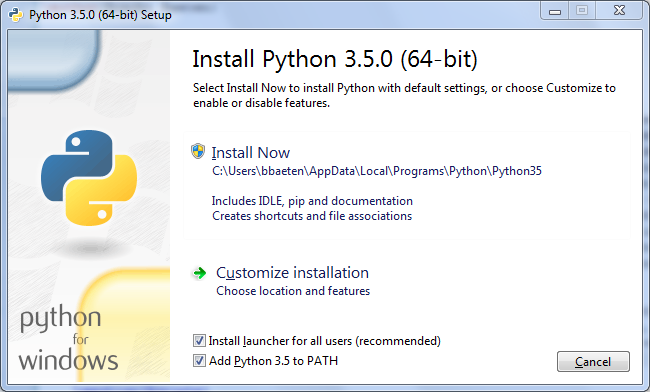
\includegraphics[scale=0.5]{Python_350_(64-bit)_Setup}
	\caption{Installatie van Python in Windows, voeg Python toe aan de PATH omgevingsvariabele}
	\label{Python_350_(64-bit)_Setup}
\end{figure}

Je kan nu al Python starten door op python.exe te klikken. Er opent een console waarin je python commando's kan invoeren (zie Figuur \ref{Python35_(64-bit)}). Typ hier bijvoorbeeld:
\begin{lstlisting}
print('Hello World!')
\end{lstlisting}

Druk op enter en je hebt je eerste python commando uitgevoerd.
\begin{figure}[htp]
	\centering
	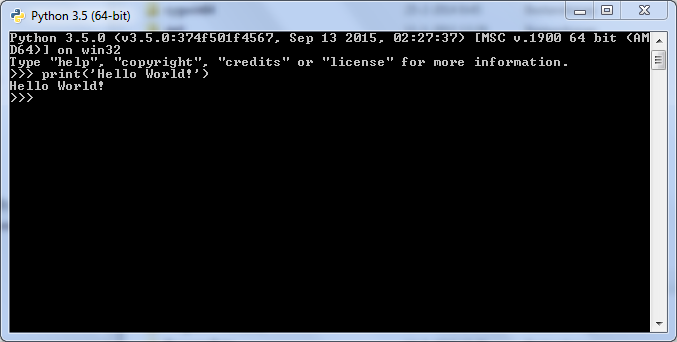
\includegraphics[scale=0.5]{Python35_(64-bit)}
	\caption{Python console met eerste commando}
	\label{Python35_(64-bit)}
\end{figure}

Python code zijn eenvoudige tekst bestanden met de extentie "\textsf{.py}". Om deze te schrijven is een goede text editor met syntax highlighting aan te raden. In Windows is \emph{notepad++} een goed, open source alternatief met syntax highlighting voor Python en een groot aantal andere talen ingebouwd. \emph{notepad++} kan worden gedownload vanop \url{https://notepad-plus-plus.org/download/}.

Omdat Python vanuit een commandline interface zal worden aangeroepen is het interessant om een deftige console te installeren. \emph{ConEmu} is een open source console emulator met gelijkenissen aan \emph{bash} op linux. Deze is te downloaden vanaf \url{http://sourceforge.net/projects/conemu/files/latest/download}. Simpelweg downloaden, unzippen in een folder naar keuze en klaar.

 	\section{Scripts}
Omdat het telkens opnieuw invoeren van commando's achter elkaar niet zo praktisch is, is het interessant om een reeks commando's op te slaan in een script en dit uit te voeren. Open een teksteditor en typ \lstinline{print('Hello World!')} en sla het bestand op als \textsf{hello\_world.py}. Om het bestand uit te voeren open je een console, navigeer naar de locatie waar je het bestand hebt opgeslagen en typ \lstinline[language=bash]{python hello\_world.py}.

\lstinputlisting{examples/hello_world.py}

	\section{Numpy, Scipy, Matplotlib} 
		
	\section{Object georiënteerd} 
	
 	\section{Modules}

\end{document}